\documentclass[border=10pt]{standalone}
\usepackage[svgnames]{xcolor}
\usepackage{amsmath}
\usepackage{pgfplots}
\pgfplotsset{compat=newest}
\usepackage[sfdefault]{FiraSans}
\usepackage{FiraMono}
\renewcommand*\familydefault{\sfdefault}
\begin{document}
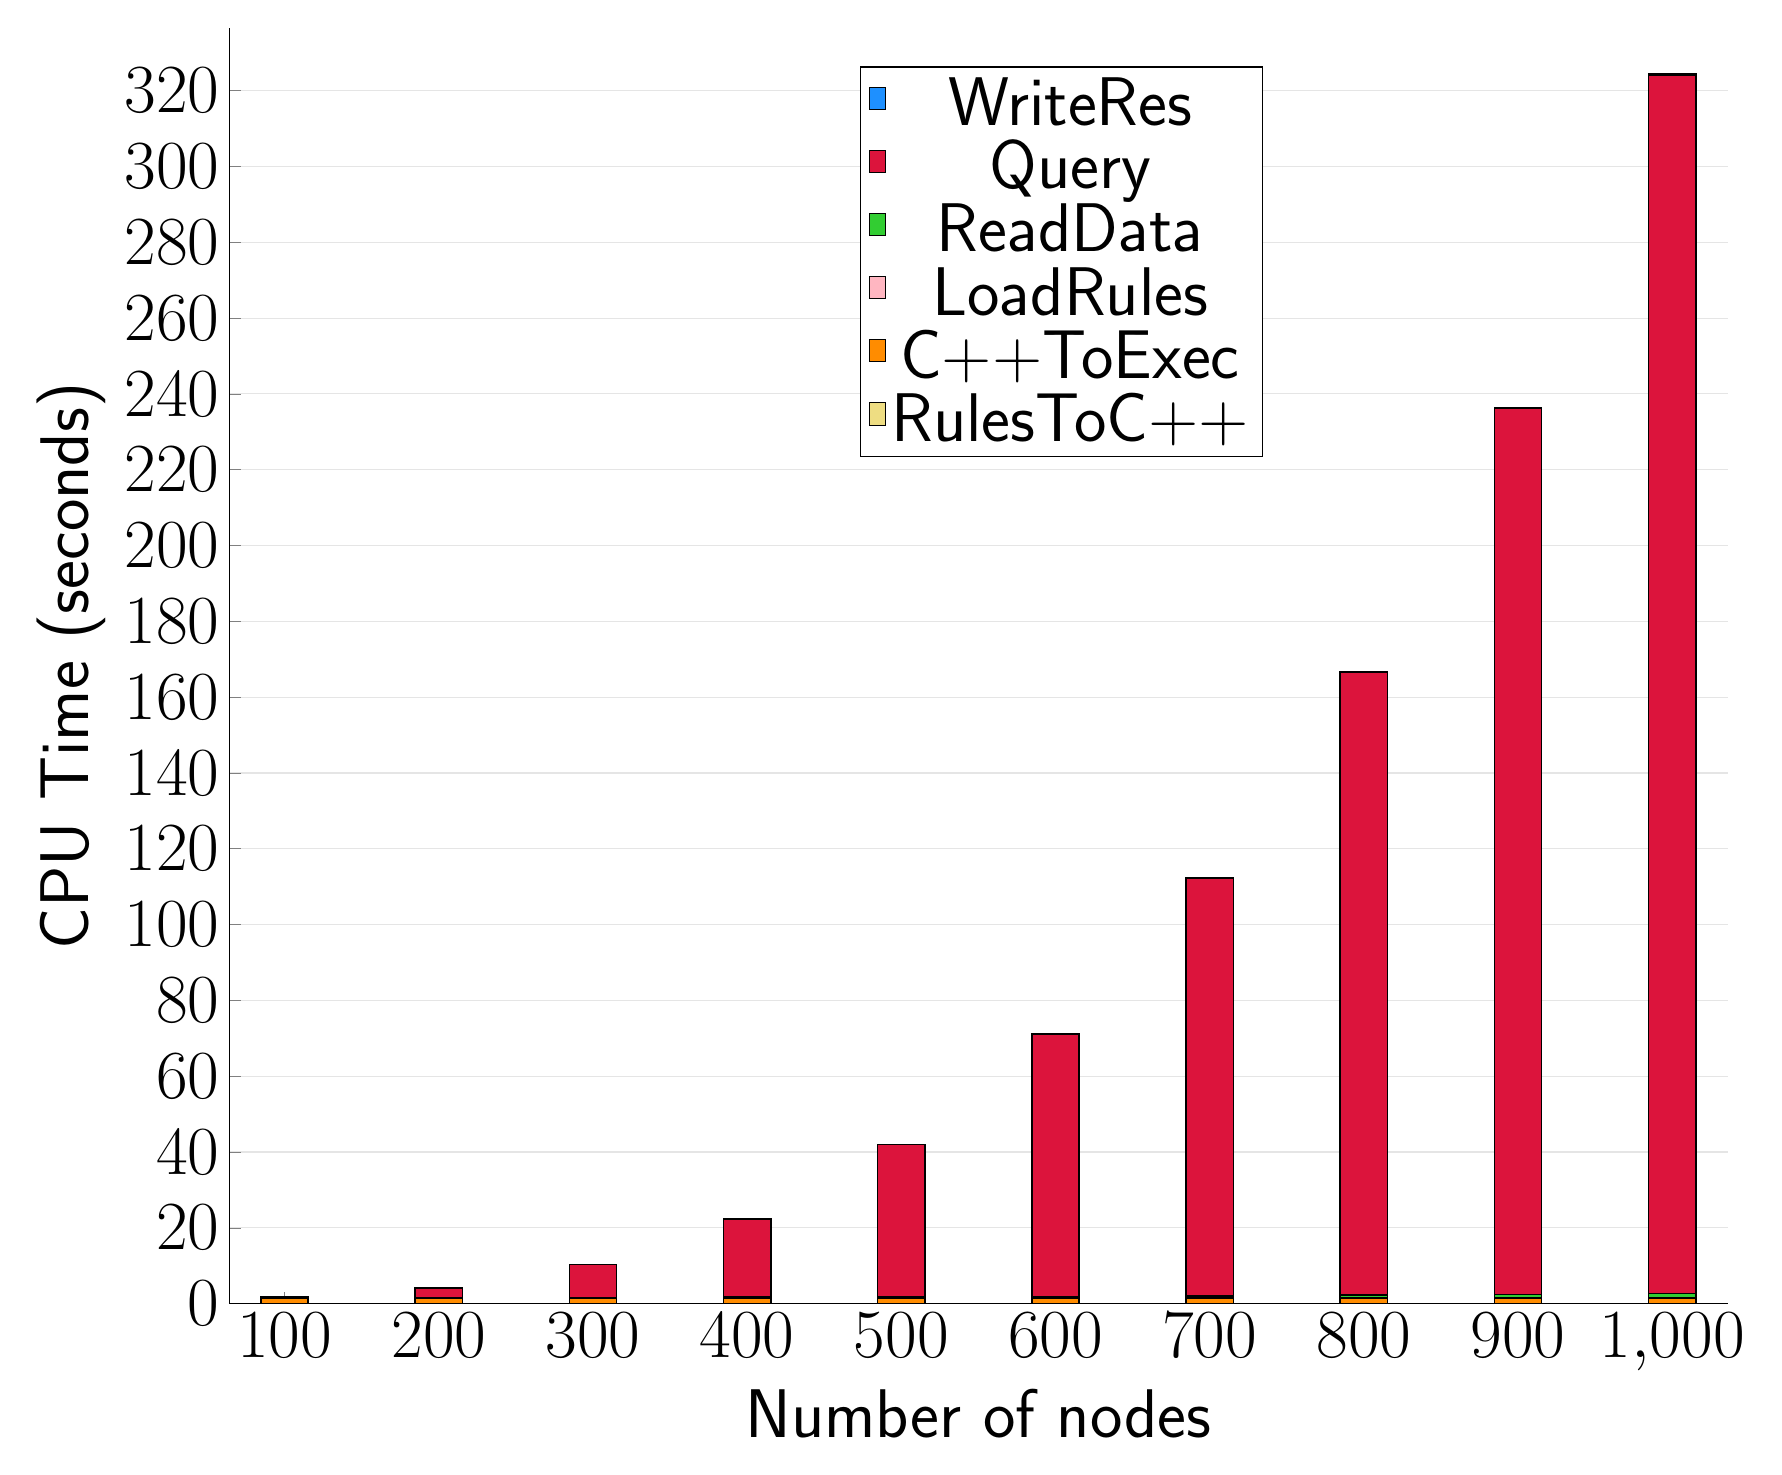
\begin{tikzpicture}
\begin{axis}[
   ybar stacked,
   width=1.7\textwidth,
   bar width=0.6cm,
   ymajorgrids, tick align=inside,
   major grid style={draw=gray!20},
   xtick=data,
   ymin=0, ymax=336.479,
   axis x line*=bottom,
   axis y line*=left,
   enlarge x limits=0.04,
   legend style={
       at={(0.69, 0.97)},
       anchor=north east,
       legend columns=1,
       font=\Huge,
   },
   ylabel={CPU Time (seconds)},
   xlabel={Number of nodes},
   label style={font=\Huge},
   tick label style={font=\Huge},
]
\addlegendimage{fill=DodgerBlue, draw=black, line width=0.2pt}
\addlegendentry{WriteRes}
\addlegendimage{fill=Crimson, draw=black, line width=0.2pt}
\addlegendentry{Query}
\addlegendimage{fill=LimeGreen, draw=black, line width=0.2pt}
\addlegendentry{ReadData}
\addlegendimage{fill=LightPink, draw=black, line width=0.2pt}
\addlegendentry{LoadRules}
\addlegendimage{fill=DarkOrange, draw=black, line width=0.2pt}
\addlegendentry{C++ToExec}
\addlegendimage{fill=LightGoldenrod, draw=black, line width=0.2pt}
\addlegendentry{RulesToC++}
\addplot +[fill=LightGoldenrod, draw=black, line width=0.55pt] coordinates {
(100, 0.004000000000000001)
(200, 0.006000000000000001)
(300, 0.0)
(400, 0.0020000000000000005)
(500, 0.0020000000000000005)
(600, 0.0)
(700, 0.0)
(800, 0.0)
(900, 0.0)
(1000, 0.0)
};
\addplot +[fill=DarkOrange, draw=black, line width=0.55pt] coordinates {
(100, 1.4780000000000002)
(200, 1.488)
(300, 1.49)
(400, 1.482)
(500, 1.484)
(600, 1.4819999999999998)
(700, 1.478)
(800, 1.4739999999999998)
(900, 1.478)
(1000, 1.472)
};
\addplot +[fill=LightPink, draw=black, line width=0.55pt] coordinates {
(100, 0.00019460000000000001)
(200, 0.00019)
(300, 0.0001796)
(400, 0.0001826)
(500, 0.00020280000000000002)
(600, 0.0002238)
(700, 0.0002058)
(800, 0.0001938)
(900, 0.00019940000000000002)
(1000, 0.00022659999999999998)
};
\addplot +[fill=LimeGreen, draw=black, line width=0.55pt] coordinates {
(100, 0.0246352)
(200, 0.06695219999999999)
(300, 0.12414019999999999)
(400, 0.2035256)
(500, 0.3081738)
(600, 0.43650859999999997)
(700, 0.5842818000000001)
(800, 0.7573714)
(900, 0.9555771999999999)
(1000, 1.176226)
};
\addplot +[fill=Crimson, draw=black, line width=0.55pt] coordinates {
(100, 0.3380854)
(200, 2.587596)
(300, 8.642992)
(400, 20.57384)
(500, 40.12352)
(600, 69.08986)
(700, 110.1858)
(800, 164.339)
(900, 233.8094)
(1000, 321.479)
};
\addplot +[fill=DodgerBlue, draw=black, line width=0.55pt] coordinates {
(100, 0.002399)
(200, 0.008863199999999998)
(300, 0.019597999999999997)
(400, 0.0342352)
(500, 0.053205199999999994)
(600, 0.07627439999999999)
(700, 0.1044962)
(800, 0.1352604)
(900, 0.170582)
(1000, 0.21060859999999998)
};
\end{axis}
\end{tikzpicture}

\end{document}
